\chapter{Selected Topics}
\label{chapter:advanced}

In this chapter we cover several selected topics of formal language theory that are related to our own models. Section \ref{section:restarting-automata} is devoted to \emph{restarting automata} \cite{O06}. Although our models are higly influenced by the theory of restarting automata, we study them from the perspective of \emph{string-rewriting systems} \cite{bookOtto93} introduced in Section \ref{section:string-rewriting-systems}. In Section \ref{section:context-rewriting-systems} we define the so-called \emph{context rewriting systems}, from which all our models are derived. We conclude this chapter by presenting some other related models in Section \ref{section:other-models}.

\section{Restarting Automata}
\label{section:restarting-automata}
\index{restarting automaton}

The main source for this section is \cite{O06}. The \index{restarting automaton}\emph{restarting automaton} was introduced in \cite{JMPV95} in order to model the so-called \index{analysis by reduction}\emph{analysis by reduction}, which is a technique used in linguistics to analyze sentences of natural languages that have a free word order. By now there are many different models of \index{restarting automaton}restarting automata, and their investigation has proved very fruitful in that they offer an opportunity to study the influence of various kinds of resources on their expressive power. Here we introduce and discuss the main variants of these automata.

\index{analysis by reduction}\emph{Analysis by reduction} is a technique used in linguistics to analyze sentences of natural languages that have a free word order. This analysis consists of a stepwise simplification of a sentence in such a way that the syntactical correctness or incorrectness of the sentence is not affected. After a finite number of steps either a correct simple sentence is obtained, or an error is detected. In the former case the given sentence is accepted as being syntactically correct; if, however, all possible sequences of simplifications yield errors, then the given sentence is not syntactically correct. In this way it is also possible to determine dependencies between various parts of the given sentence, and to disambiguate between certain morphological ambiguities contained in the sentence.

As illustrated by Jančar et al. (e.\,g.\ \cite{JMPV99}) the \index{restarting automaton}restarting automaton was invented to model the \index{analysis by reduction}analysis by reduction. In fact, many aspects of the work on restarting automata are motivated by the basic tasks of computational linguistics. The notions developed in the study of restarting automata give a rich taxonomy of constraints for various models of analyzers and parsers. Already several programs are being used in Czech and German (corpus) linguistics that are based on the idea of restarting automata.

As defined in \cite{JMPV95} the \index{restarting automaton}\emph{restarting automaton} is a nondeterministic machine model that processes strings which are stored in a list (or a ‘rubber’ \index{tape}tape) with end \index{marker}markers. It has a finite control, and it has a \index{read/write window}read/write window with a finite look-ahead working on the list of symbols. The \index{restarting automaton}restarting automaton can only perform two kinds of operations: \index{transition step!move-right} \emph{move-right transitions}, which shift the \index{read/write window}read/write window one position to the right, thereby changing the actual state, and combined \index{transition step!delete/restart}\emph{delete/restart transitions}, which delete some symbols from the \index{read/write window}read/write window, place this window over the left end of the list, and put the automaton back into its \index{state!initial}initial state. Hence, after performing a \index{transition step!delete/restart}delete/restart transition a \index{restarting automaton}restarting automaton has no way to remember that it has already performed some steps of a computation. Further, by each application of a \index{transition step!delete/restart}delete/restart transition the list is shortened. It follows that \index{restarting automaton}restarting automata are linearly space-bounded.

Subsequently Jančar et al. extended their model in various ways. Instead of simply deleting some symbols from the actual content of the \index{read/write window}read/write window during a \index{transition step!delete/restart}delete/restart transition, a \index{restarting automaton!with rewriting}restarting automaton \emph{with rewriting} has combined \index{transition step!rewrite/restart}\emph{rewrite/restart} transitions that replace the content of the \index{read/write window}read/write window by a shorter string \cite{JMPV97}. Further, the use of \index{auxiliary symbol}auxiliary (that is, non-input) symbols was added to the model in \cite{JMPV98}, which yields the so-called \index{$\RWW$-automaton}\emph{$\RWW$-automaton}. Also in \cite{JMPV98} the \index{transition step!restart}restart transition was separated from the \index{transition step!rewrite}rewrite transition so that, after performing a rewrite step, the automaton can still read the remaining part of the tape before performing a \index{transition step!restart}restart transition. This gives the so-called \index{$\RRWW$-automaton}\emph{$\RRWW$-automaton}, which is required to execute exactly one \index{transition step!rewrite}rewrite transition between any two \index{transition step!restart}restart transitions. In addition, various notions of \index{restarting automaton!monotone}\emph{monotonicity} have been discussed for the various types of \index{restarting automaton}restarting automata. It turned out that monotone \index{$\RWW$-automaton}$\RWW$- and \index{$\RRWW$-automaton}$\RRWW$-automata accept exactly the \index{language!context-free}context-free languages, and that all the various types of monotone deterministic \index{$\RWW$-automaton}$\RWW$- and \index{$\RRWW$-automaton}$\RRWW$-automata accept exactly the \index{language!context-free!deterministic}deterministic context-free languages. Finally, \index{transition step!move-left}\emph{move-left transitions} were added to the \index{restarting automaton}restarting automaton, which gave the so-called \index{restarting automaton!two-way}\emph{two-way restarting automaton} \index{$\RLWW$-automaton}($\RLWW$-automaton) \cite{P01}. This automaton can first scan its tape completely, and then move left to apply a rewrite transition to some factor of the \index{tape}tape content.

In defining the \index{restarting automaton}restarting automaton and its main variants we will not follow the historical development outlined above, but we will first present the most general model, the \index{$\RLWW$-automaton}$\RLWW$-automaton, and then describe the other variants as restrictions thereof.

As indicated above a \index{restarting automaton}restarting automaton is a nondeterministic machine model that has a finite control and a \index{read/write window}read/write window that works on a list of symbols delimited by end \index{marker}markers (see Figure \ref{figure:restarting_automaton}).

\begin{figure}[htp]
\centering
\includegraphics[scale=1.0]{img/restarting_automaton.eps}
\caption[Schematic representation of a restarting automaton.]
{Schematic representation of a restarting automaton.}
\label{figure:restarting_automaton}
\end{figure}

Formally, a \index{restarting automaton!two-way}\emph{two-way restarting automaton}, \index{$\RLWW$-automaton}$\RLWW$-automaton for short, is a one-tape machine described by an $8$-tuple $M = (Q, \Sigma, \Gamma, \cent, \$, q_0, k, \delta)$, where $Q$ is a finite set of \index{state}states, $\Sigma$ is a finite \index{alphabet!input}input alphabet, $\Gamma$ is a finite \index{alphabet!tape}tape alphabet containing $\Sigma$, \index{$\cent$}\index{$\$$}$\cent, \$ \notin \Gamma$ are symbols that serve as \index{marker}\emph{markers} (or \index{sentinel}\emph{sentinels}) for the left and right border of the work space, respectively, $q_0 \in Q$ is the \index{state!initial}initial state, $k \ge 1$ is the size of the \index{read/write window}\emph{read/write window}, and $$\delta: Q \times \mathfrak{PC}^{(k)} \to \mathcal{P}((Q \times (\{\MVR, \MVL\} \cup \mathfrak{PC}^{\le (k-1)})) \cup \{\Restart, \Accept\})$$ is the \index{transition!relation}\emph{transition relation}. Here $\mathfrak{PC}^{(k)}$ is the set of \index{read/write window!possible contents}\emph{possible contents} of the read/write window of $M$, where $$\mathfrak{PC}^{(i)} = (\cent \cdot \Gamma^{i-1}) \cup \Gamma^i \cup (\Gamma^{\le i-1} \cdot \$) \cup (\cent \cdot \Gamma^{\le i-2} \cdot \$)\ \ (i \ge 0),$$ and $$\Gamma^{\le n} = \bigcup_{i=0}^n \Gamma^i \text{ and } \mathfrak{PC}^{\le (k-1)} = \bigcup_{i=0}^{k-1}\mathfrak{PC}^{(i)}.$$

The \index{transition!relation}transition relation describes five different types of \index{transition step}transition steps:

\begin{enumerate}
\item A \emph{move-right step} is of the form \index{$\MVR$}$(q', \MVR) \in \delta(q, u)$, where $q, q' \in Q$ and $u \in \mathfrak{PC}^{(k)}$, $u \neq \$$. If $M$ is in state $q$ and sees the string $u$ in its read/write window, then this move-right step causes $M$ to shift the read/write window one position to the right and to enter state $q'$. However, if the content $u$ of the read/write window is only the symbol $\$$, then no shift to the right is possible.
\item A \index{transition step!move-left}\emph{move-left step} is of the form \index{$\MVL$}$(q', \MVL) \in \delta(q, u)$, where $q, q' \in Q$ and $u \in \mathfrak{PC}^{(k)}$ does not begin with the symbol $\cent$. It causes $M$ to shift the \index{read/write window}read/write window one position to the left and to enter state $q'$. This, however, is only possible if the window is not already at the left end of the tape.
\item A \index{transition step!rewrite}\emph{rewrite step} is of the form $(q', v) \in \delta(q, u)$, where $q, q' \in Q$ and $u \in \mathfrak{PC}^{(k)}$, $u \neq \$$, and $v \in \mathfrak{PC}^{\le (k-1)}$ such that $|v| < |u|$. It causes $M$ to replace the content of $u$ of the \index{read/write window}read/write window by the string $v$, thereby shortening the tape, and to enter state $q'$. Further, the \index{read/write window}read/write window is placed immediately to the right of the string $v$. However, some additional restrictions apply in that the border \index{marker}markers  $\cent$ and $\$$ must not disappear from the tape nor that new occurrences of these markers are created. Further, the \index{read/write window}read/write window must not move across the right border \index{marker}marker $\$$, that is, if the string $u$ ends in $\$$, then so does the string $v$, and after performing the rewrite operation, the \index{read/write window}read/write window is placed on the $\$$-symbol.
\item A \index{transition step!restart}\emph{restart step} is of the form \index{$\Restart$}$\Restart \in \delta(q, u)$, where $q \in Q$ and $u \in \mathfrak{PC}^{(k)}$. It causes $M$ to place its \index{read/write window}read/write window over the left end of the tape, so that the first symbol it sees is the left border \index{marker}marker $\cent$, and to reenter the \index{state!initial}initial state $q_0$.
\item An \index{transition step!accept}\emph{accept step} is of the form \index{$\Accept$}$\Accept \in \delta(q, u)$, where $q \in Q$ and $u \in \mathfrak{PC}^{(k)}$. It causes $M$ to halt and accept.
\end{enumerate}

If $\delta(q, u) = \emptyset$ for some $q \in Q$ and $u \in \mathfrak{PC}^{(k)}$, then $M$ necessarily halts, and we say that $M$ \emph{rejects} in this situation. Further, the letters in $\Gamma \backslash \Sigma$ are called \index{auxiliary symbol}\emph{auxiliary symbols}.

A \index{configuration}\emph{configuration} of $M$ is a string $\alpha q \beta$, where $q \in Q$, and either $\alpha = \lambda$ and $\beta \in \{\cent\} \cdot \Gamma^* \cdot \{\$\}$ or $\alpha \in \{\cent\} \cdot \Gamma^*$ and $\beta \in \Gamma^* \cdot \{\$\}$; here $q \in Q$ represents the \index{state!current}current state, $\alpha \beta$ is the current content of the \index{tape}tape, and it is understood that the \index{read/write window}read/write window contains the first $k$ symbols of $\beta$ or all of $\beta$ when $|\beta| \le k$. A \index{configuration!restarting}\emph{restarting configuration} is of the form $q_0 \cent w \$$, where $w \in \Gamma^*$; if $w \in \Sigma^*$, then $q_0 \cent w \$$ is an \index{configuration!initial}\emph{initial configuration}. Thus, initial configurations are a particular type of restarting configurations. Further, we use \index{$\Accept$}$\Accept$ to denote the \index{configuration!accepting}\emph{accepting configurations}, which are those configurations that $M$ reaches by executing an \index{$\Accept$}$\Accept$ instruction. A configuration of the form $\alpha q \beta$ such that $\delta(q, \beta_1) = \emptyset$, where $\beta_1$ is the current content of the \index{read/write window}read/write window, is a \index{configuration!rejecting}\emph{rejecting configuration}. A \index{configuration!halting}\emph{halting configuration} is either an \index{configuration!accepting}accepting or a \index{configuration!rejecting}rejecting configuration.

In general, the automaton $M$ is \index{restarting automaton!nondeterministic}\emph{nondeterministic}, that is, there can be two or more instructions with the same left-hand side $(q, u)$, and thus, there can be more than one \index{computation}computation for an input word. If this is not the case, the automaton is \index{restarting automaton!deterministic}\emph{deterministic}. We use the prefix \index{$\detPrefix$}$\detPrefix$ to denote deterministic classes of restarting automata.

We observe that any finite \index{computation}computation of a \index{restarting automaton!two-way}two-way restarting automaton $M$ consists of certain phases. A phase, called a \index{cycle}\emph{cycle}, starts in a \index{configuration!restarting}restarting configuration, the head moves along the \index{tape}tape performing \index{$\MVR$}$\MVR$, \index{$\MVL$}$\MVL$, and \index{$\Rewrite$}$\Rewrite$ operations until a \index{$\Restart$}$\Restart$ operation is performed and thus a new \index{configuration!restarting}restarting configuration is reached. If no further \index{$\Restart$}$\Restart$ operation is performed, any finite computation necessarily finishes in a \index{configuration!halting}halting configuration -- such a phase is called a \index{tail}\emph{tail}. We require that $M$ performs \emph{exactly one} \index{$\Rewrite$}$\Rewrite$ operation during any cycle -- thus each new phase starts on a shorter word than the previous one. During a \index{tail}tail at most one \index{$\Rewrite$}$\Rewrite$ operation may be executed. By $\vdash_M$ we denote the execution of a complete \index{cycle}cycle, and $\vdash_M^{c^*}$ is the reflexive and transitive closure of this relation. It can be seen as the \index{rewriting relation}\emph{rewrite relation} that is realized by $M$ on the set of restarting configurations.

An input $w \in \Sigma^*$ is accepted by $M$, if there exists a \index{computation}computation of $M$ which starts with the \index{configuration!initial}initial configuration  $q_0 \cent w \$$, and which finally ends with executing an \index{$\Accept$}$\Accept$ instruction.

Given an input of length $n$, and $\RLWW$-automaton can execute at most $n$ cycles. Thus, we have the following result, where $\classNP$ and $\classP$ denote the well-known complexity classes, and $\DCSL$ denotes the class of \emph{deterministic context-sensitive languages}, that is, the space complexity $\classDSPACE(n)$.

\begin{proposition}
\begin{eqnarray*}
\calL{\RLWW} & \subseteq & \classNP \cap \CSL,\\
\calL{\detRLWW} & \subseteq & \classP \cap \DCSL.
\end{eqnarray*}
\end{proposition}

In the following we restate some basic facts about \index{computation}computations of \index{restarting automaton}restarting automata.

\index{error preserving theorem}
\begin{proposition}[Error Preserving Property]\label{proposition:error-preserving-rlww}
Let $M$ be an \index{$\RLWW$-automaton}$\RLWW$-automaton, and let $u, v$ be words over its \index{alphabet!input}\emph{input} alphabet $\Sigma$. If $q_0 \cent u \$ \vdash_M^{c^*} q_0 \cent v \$$ holds and $u \notin L(M)$, then $v \notin L(M)$, either.
\end{proposition}

\index{correctness preserving theorem}
\begin{proposition}[Correctness Preserving Property]\label{proposition:correctness-preserving-rlww}
Let $M$ be an \index{$\RLWW$-automaton}$\RLWW$-automaton, and let $u, v$ be words over its \index{alphabet!input}\emph{input} alphabet $\Sigma$. If $q_0 \cent u \$ \vdash_M^{c^*} q_0 \cent v \$$ is an initialsegment of an \emph{accepting} computation of $M$, then $v \in L(M)$.
\end{proposition}

Each \index{cycle}cycle of each \index{computation}computation of an \index{$\RLWW$-automaton}$\RLWW$-automaton $M$ consists of three phases: first $M$ scans its tape performing \index{$\MVR$}$\MVR$- and \index{$\MVL$}$\MVL$-instructions, then it executes a \index{$\Rewrite$}$\Rewrite$ step, and finally it scans its tape again performing \index{$\MVR$}$\MVR$- and \index{$\MVL$}$\MVL$-steps. Hence, in the first and the last phase of each cycle $M$ behaves like a nondeterministic two-way finite-state acceptor ($2$-$\NFA$). In an analogy to the proof that the language accepted by a $2$-$\NFA$ is regular (see e.\,g.\ \cite{HopcroftMotwaniUllman07}), the following result can be established. Here a \index{restarting automaton}restarting automaton is called an \index{$\RRWW$-automaton}\emph{$\RRWW$-automaton} if it does not use any \index{$\MVL$}$\MVL$-transitions. Thus, in each cycle an \index{$\RRWW$-automaton}$\RRWW$-automaton can scan its tape only once from left to right.

\begin{theorem}
Let $M_L = (Q_L, \Sigma, \Gamma, \cent, \$, q_0, k, \delta_L)$ be an \index{$\RLWW$-automaton}$\RLWW$-automaton. Then there exists an \index{$\RRWW$-automaton}$\RRWW$-automaton $M_R = (Q_R, \Sigma, \Gamma, \cent, \$, q_0, k, \delta_R)$ such that, for all $u, v \in \Gamma^*$, $$q_0 \cent u \$ \vdash_{M_L}^c q_0 \cent v \$ \text{ if and only if } q_0 \cent u \$ \vdash_{M_R}^c q_0 \cent v \$,$$ and the languages $L(M_L)$ and $L(M_R)$ coincide.
\end{theorem}

Thus, as far as \index{restarting automaton!nondeterministic}nondeterministic restarting automata are concerned, the \index{$\MVL$}$\MVL$-instruction is not needed. However, this does not hold for \index{restarting automaton!deterministic}deterministic restarting automata. For \index{$\RRWW$-automaton}$\RRWW$-automata we have the following normalization result, which is easily proved by using standard techniques from automata theory.

\begin{lemma}
Each \index{$\RRWW$-automaton}$\RRWW$-automaton $M$ is equivalent to an \index{$\RRWW$-automaton}$\RRWW$-automaton $M'$ that satisfies the following additional restriction:
\begin{enumerate}
\item[(*)] $M'$ makes an \index{transition step!accept}accept or a \index{transition step!restart}restart step only when it sees the right border \index{marker}marker $\$$ in its \index{read/write window}read/write window.
\end{enumerate}
\end{lemma}

This lemma means that in each \index{cycle}cycle of each \index{computation}computation and also during the \index{tail}tail of each \index{computation!accepting}accepting computation the \index{read/write window}read/write window moves all the way to the right before a restart is made, respectively, before the machine halts and accepts.

Based on this fact each \index{cycle}cycle (and also the \index{tail}tail) of a \index{computation}computation of an \index{$\RRWW$-automaton}$\RRWW$-automaton consists of three phases. Accordingly, the transition relation of an \index{$\RRWW$-automaton}$\RRWW$-automaton can be described through a sequence of so-called \index{meta-instruction}\emph{meta-instructions} of the form $(E_1, u \to v, E_2)$, where $E_1$ and $E_2$ are \index{language!regular}regular languages, called the \index{constraint}\emph{regular constraints} of this instruction, and $u$ and $v$ are strings such that $|u| > |v|$. The rule $u \to v$ stands for a \index{$\Rewrite$}$\Rewrite$ step of the \index{$\RRWW$-automaton}$\RRWW$-automaton $M$ considered. On trying to execute this \index{meta-instruction}meta-instruction $M$ will get stuck (and so reject) starting from the \index{configuration}configuration $q_0 \cent w \$$, if $w$ does not admit a factorization of the form $w = w_1 u w_2$ such that $\cent w_1 \in E_1$ and $w_2 \$ \in E_2$. On the other hand, if $w$ does have a factorization of this form, then one such factorization is chosen nondeterministically, and $q_0 \cent w \$$ is transformed into $q_0 \cent w_1 v w_2 \$$. In order to describe the \index{tail}tails of \index{computation!accepting}accepting computations we use \index{meta-instruction}meta-instructions of the form \index{$\Accept$}$(\cent \cdot E \cdot \$, \Accept)$, where the strings from the \index{language!regular}regular language $E$ are accepted by $M$ in \index{tail}tail \index{computation}computations.

\begin{example}
Let $M$ be the $\RRWW$-automaton with input alphabet $\Sigma = \{a, b, c, d\}$ and without auxiliary symbols that is described by the following sequence of meta-instructions:
\begin{center}
\begin{tabular}{c c c c c c c}
$(1)$ & $(\cent \cdot a^*,$ & $ab \to \lambda,$ & $b^* \cdot c \$),$ & \hspace{1cm} $(3)$ & $(\cent c \$,$ & $\Accept),$ \\
$(2)$ & $(\cent \cdot a^*,$ & $abb \to \lambda,$ & $b^* \cdot d \$),$ & \hspace{1cm} $(4)$ & $(\cent d \$,$ & $\Accept).$ \\
\end{tabular}
\end{center}
It is easily seen that $L(M) = \{a^n b^n c \mid n \ge 0\} \cup \{a^n b^{2n} d \mid n \ge 0\}$.
\end{example}

Finally, we introduce some restricted types of restarting automata. A \index{restarting automaton}restarting automaton is called an \index{$\RWW$-automaton}\emph{$\RWW$-automaton} if it makes a \index{transition step!restart}restart immediately after performing a \index{transition step!rewrite}rewrite operation. In particular, this means that it cannot perform a \index{transition step!rewrite}rewrite step during the \index{tail}tail of a \index{computation}computation.

A \index{cycle}cycle of a \index{computation}computation of an \index{$\RWW$-automaton}$\RWW$-automaton $M$ consists of two phases only. Accordingly, the transition relation of an $\RWW$-automaton can be described by a finite sequence of \index{meta-instruction}\emph{meta-instructions} of the form $(E, u \to v)$, where $E$ is a \index{language!regular}regular language, and $u$ and $v$ are strings such that $|u| > |v|$, and \index{meta-instruction}meta-instructions of the form \index{$\Accept$}$(\cent \cdot E \cdot \$, \Accept)$ for describing \index{tail}tail \index{computation}computations.

An \index{$\RLWW$-automaton}$\RLWW$-automaton is called an \index{$\RLW$-automaton}\emph{$\RLW$-automaton} if its \index{alphabet!tape}tape alphabet $\Gamma$ coincides with its \index{alphabet!input}input alphabet $\Sigma$, that is, if no \index{auxiliary symbol}auxiliary symbols are available. It is an \index{$\RL$-automaton}\emph{$\RL$-automaton} if it is an \index{$\RLW$-automaton}$\RLW$-automaton for which the right-hand side $v$ of each \index{$\Rewrite$}$\Rewrite$ step $(q', v) \in \delta(q, u)$ is a \index{subword!scattered}scattered subword of the left-hand side $u$. Analogously, we obtain \index{$\RRW$-automaton}$\RRW$- and \index{$\RR$-automaton}$\RR$-automata from the \index{$\RRWW$-automaton}$\RRWW$-automaton and \index{$\RW$-automaton}$\RW$- and \index{$\R$-automaton}$\R$-automata from the \index{$\RWW$-automaton}$\RWW$-automaton, respectively.

It can be shown that $\calL{\R}$ contains languages that are not \index{language!context-sensitive!growing}\emph{growing context-sensitive}. Hence, already the \index{$\R$-automaton}$\R$-automaton has a fairly large expressive power.

We conclude this section with the notion of monotonicity for restarting automata (introduced in \cite{JMPV97}). Here we consider a slightly more general notion, which is taken from \cite{JMPV07}. Let $M$ be an \index{$\RLWW$-automaton} $\RLWW$-automaton. Each \index{computation}computation of $M$ can be described by a sequence of \index{cycle}cycles $C_1, C_2, \ldots, C_n$, where $C_n$ is the last cycle, which is followed by the \index{tail}tail of the \index{computation}computation. Each \index{cycle}cycle $C_i$ of this \index{computation}computation contains a unique \index{configuration}configuration of the form $\cent x q u y \$$ such that $q$ is a \index{state}state and $(q', v) \in \delta(q, u)$ is the \index{$\Rewrite$}$\Rewrite$ step that is applied during this cycle. By $D_r(C_i)$ we denote the \index{cycle!right distance}\emph{right distance} $|u y \$|$ of this cycle, and $D_l(C_i)$ is the \index{cycle!left distance}\emph{left distance} $|\cent x|$ of this cycle. The sequence of cycles $C_1, C_2, \ldots, C_n$ is called \emph{monotone} if $D_r(C_1) \ge D_r(C_2) \ge \ldots \ge D_r(C_n)$ holds. A computation of $M$ is called \index{computation!monotone}\emph{monotone} if the corresponding sequence of cycles is monotone. Observe that the tail of the computation is not taken into account here. Finally, the \index{$\RLWW$-automaton}$\RLWW$-automaton $M$ is called \index{restarting automaton!monotone}\emph{monotone} if each of its \index{computation}computations that starts from an \index{configuration!initial}initial configuration is monotone.

Here we want to compare the expressive power of the various types of \index{restarting automaton!monotone}monotone restarting automata to each other. We use the prefix \index{$\monPrefix$}$\monPrefix$ to denote the classes of monotone restarting automata.

All variants of 
\index{restarting automaton!deterministic}\index{restarting automaton!monotone}deterministic monotone restarting automata obtained from the \index{$\RRWW$-automaton}$\RRWW$-automaton coincide in their expressive power:

\index{$\DCFL$}\index{$\R$-automaton}\index{$\RR$-automaton}\index{$\RW$-automaton}\index{$\RRW$-automaton}\index{$\RWW$-automaton}\index{$\RRWW$-automaton}
\begin{theorem}
For all types $\X \in \{\R, \RR, \RW, \RRW, \RWW, \RRWW\}$, $$\calL{\detmonX} = \DCFL.$$
\end{theorem}

\noindent However, it can be shown that \index{$\RL$-automaton} \index{$\RLWW$-automaton} $\DCFL \subset \calL{\detmonRL} \subseteq \calL{\detmonRLWW}$.

For nondeterministic restarting automata it turns out that the use of \index{auxiliary symbol}auxiliary symbols is necessary to obtain a characterization of the class of \index{language!context-free}context-free languages.

\index{$\CFL$}\index{$\RLWW$-automaton}\index{$\RRWW$-automaton}\index{$\RWW$-automaton}
\begin{theorem}
For all types $\X \in \{\RLWW, \RRWW, \RWW\}$, $$\calL{\monX} = \CFL.$$
\end{theorem}

\section{String-Rewriting Systems}
\label{section:string-rewriting-systems}

As we have already mentioned we study our models from the perspective of \emph{string-rewriting systems}. The main source for this section is \cite{bookOtto93} (although here we use a slightly different notation). In Section \ref{subsection:mcnaughton-families} we cover \emph{McNaughton Families of Languages} \cite{Beaudry2003} and in Section \ref{section:delimited-string-rewriting-systems} we give a short overview of \emph{delimited string-rewriting systems} \cite{Eyraud2007}.

\begin{definition}[String-rewriting systems \cite{bookOtto93}]
Let $\Sigma$ be a finite alphabet.

\begin{enumerate}
\item A \index{string-rewriting system}\emph{string-rewriting system} (\index{$\SRS$}$\SRS$) $R$ on $\Sigma$ is a set of \index{rule!rewrite}\emph{(rewrite) rules} $(l \to r)$, where $l, r \in \Sigma^*$. The set $\{l \in \Sigma^* \mid \exists r \in \Sigma^*: (l \to r) \in R\}$ is called the \index{domain}\emph{domain} of $R$ and is denoted \index{$\dom(R)$}$\dom(R)$. The set $\{r \in \Sigma^* \mid \exists l \in \Sigma^*: (l \to r) \in R\}$ is called the \index{range}\emph{range} of $R$ and is denoted \index{$\rng(R)$}$\rng(R)$. If $R$ is finite, then the \emph{size} of $R$ is defined to be $\sum_{(l \to r) \in R}(|l| + |r|)$ and is denoted \index{$\|R\|$}$\|R\|$. The \emph{width} of rule $(l \to r) \in R$ is $|l| + |r|$.
\item If $R$ is a string-rewriting system on $\Sigma$, then the \index{reduction relation!single-step}\emph{single-step reduction relation} on $\Sigma^*$, that is induced by $R$ is defined as follows: for any $u, v \in \Sigma^*$, $u \Rightarrow_R v$ if and only if there exists $(l \to r) \in R$ such that for some $x, y \in \Sigma^*$, $u = xly$ and $v = xry$. The \index{reduction relation}\emph{reduction relation} on $\Sigma^*$ induced by $R$ is the reflexive and transitive closure of $\Rightarrow_R$ and is denoted by $\Rightarrow^*_R$.
\item For a string $u \in \Sigma^*$, if there exists a string $v$ such that $u \Rightarrow_R v$ holds, then $u$ is called \emph{reducible} modulo $R$, $v$ is a \emph{direct descendant} of $u$, and $u$ is a \emph{direct ancestor} of $v$. If such a string $v$ does not exist, then $u$ is called \emph{irreducible} modulo $R$. By \index{$\Delta_R^*(u)$}$\Delta_R^*(u)$ we denote the set of all descendants of $u$, that is, $\Delta_R^*(u) := \{v \mid u \Rightarrow_R^* v\}$, \index{$\nabla_R^*(v)$}$\nabla_R^*(v)$ is the set of all ancestors of $v$, that is, $\nabla_R^*(v) := \{u \mid u \Rightarrow_R^* v\}$, and by \index{$\IRR(R)$}$\IRR(R)$ we denote the set of all irreducible strings modulo $R$.
\end{enumerate}
\end{definition}

\begin{definition}[\cite{bookOtto93}]
Let $R$ be a string-rewriting system on $\Sigma$. We say that $R$ is:
\begin{enumerate}
\item \index{string-rewriting system!terminating}\emph{terminating} or \index{string-rewriting system!noetharian}\emph{noetherian} if there is no infinite sequence of reduction steps $w_1 \Rightarrow_R w_2 \Rightarrow_R w_3 \Rightarrow_R \ldots$,
\item \index{string-rewriting system!locally confluent}\emph{locally confluent} if, for all $u, v, w \in \Sigma^*$, $u \Rightarrow_R v$ and $u \Rightarrow_R w$ imply that there exists some $z \in \Sigma^*$ such that $v \Rightarrow_R^* z$ and $w \Rightarrow_R^* z$ hold,
\item \index{string-rewriting system!confluent}\emph{confluent} if, for all $u, v, w \in \Sigma^*$, $u \Rightarrow_R^* v$ and $u \Rightarrow_R^* w$ imply that there exists some $z \in \Sigma^*$ such that $v \Rightarrow_R^* z$ and $w \Rightarrow_R^* z$ hold,
\item \index{string-rewriting system!convergent}\emph{convergent} if it is both noetherian and confluent,
\item \index{string-rewriting system!generalized monadic}\emph{generalized monadic}, if $|l| \ge |r|$ and $|r|\le 1$ for each rule $(l \to r)\in R$,
\item \index{string-rewriting system!monadic}\emph{monadic}, if $|l| > |r|$ and $|r|\le 1$ for each rule $(l \to r)\in R$,
\item \index{string-rewriting system!length-reducing}\emph{length-reducing}, if for each rule $(l \to r) \in R: |l| > |r|$. 
\item \index{string-rewriting system!non-increasing}\emph{non-increasing}, if for each rule $(l \to r) \in R: |l| \ge |r|$. 
\item \index{string-rewriting system!weight-reducing}\emph{weight-reducing}, if there exists a so-called \index{weight function}\emph{weight function} $f: \Sigma \to \mathsf{N}$, such that for each rule $(l \to r) \in R: f^*(l) > f^*(r)$, where $f^*: \Sigma^* \to \mathsf{N}$ is defined inductively as: $f^*(\lambda) = 0$, $f^*(xa) = f^*(x) + f(a)$ for all $x \in \Sigma^*, a \in \Sigma$.

Note that the length-reducing string-rewriting systems represent only a special case of the more general weight-reducing string-rewriting systems. To see this just consider the following weight function: $f(a) := 1$ for all $a \in \Sigma$.

Also note that every weight-reducing string-rewriting system is noetherian.
\end{enumerate}
\end{definition}

\begin{lemma}[\cite{bookOtto93}]
If $R$ is a finite string-rewriting system on alphabet $\Sigma$, then the set $\IRR(R)$ of irreducible strings with respect to $R$ is a regular language; furthermore, a finite automaton for $\IRR(R)$ can be constructed in a polynomial time from $R$.
\end{lemma}

In the literature string-rewriting systems are also known as \index{semi-Thue system}\emph{semi-Thue systems}. A string-rewriting system $R$ with the property that $(l \to r) \in R$ implies $(r \to l) \in R$ is also called a \index{Thue system}\emph{Thue system} (after the Norwegian mathematician and logician Axel Thue who introduced it in 1914). For a Thue system $R$, the single-step reduction relation $\Rightarrow_R$ is symmetric, so that the reduction relation $\Rightarrow^*_R$ coincides with the \index{Thue congruence}\emph{Thue congruence} $\Leftrightarrow^*_R$, where $\Leftrightarrow_R$ is defined as $\Rightarrow_R \cup \Rightarrow_R^{-1}$.

The reason that the relation $\Leftrightarrow^*_R$ is called a ``congruence'' relation is that it is an equivalence relation that is compatible with respect to concatenation of strings. For a convergent system $R$, the set $\IRR(R)$ of irreducible strings is a complete set of unique representatives for the Thue congruence $\Leftrightarrow^*_R$ (see, e.\,g.,~\cite{bookOtto93}).

While it is undecidable in general whether a finite string-rewriting system is confluent (see, e.\,g.,~\cite{bookOtto93}), confluence is a decidable property for finite string-rewriting systems that are terminating. Let $R$ be a string-rewriting system on~$\Sigma$. If there are two rules $(l \to r)$ and $(l' \to r')$ in $R$ such that $l = ul'v$ for some $u,v\in\Sigma^*$, then the word $l$ can be rewritten by either of the two rules: $l \Rightarrow_R r$ and $l =ul'v\Rightarrow_R ur'v$. If the system $R$ is to be confluent, then the words $r$ and $ur'v$ must have a common descendant. Accordingly, the pair $(r,ur'v)$ is called a \index{critical pair}\emph{critical pair} of~$S$. Furthermore, if $l = uv$ and $l'=vw$ for some words $u,v,w\in\Sigma^+$, then the word $uvw$ can be rewritten by either rule: $uvw= l w\Rightarrow_R rw$ and $uvw =ul'\Rightarrow_R ur'$. Hence, also $(rw,ur')$ is  a \index{critical pair}\emph{critical pair} of~$R$.

\begin{proposition}\label{PropCon}{\rm \cite{KnBe70}}
A terminating string-rewriting system is confluent if and only if, for each critical pair $(p,q)$ of $R$, $p$ and $q$ have a common descendant mod~$R$. 
\end{proposition}

If $R$ is finite, then it has only finitely many critical pairs, which can be computed. Hence, it follows immediately that confluence is decidable for finite terminating string-rewriting systems.

String-rewriting systems play a central part in the definition of the so called \index{language!Church-Rosser}\emph{Church-Rosser languages} (\index{$\CRL$}$\CRL$). A language $L \subseteq \Sigma^*$ is called a \emph{Church-Rosser language}, if it consists of those strings $w \in \Sigma^*$ that, placed within the context $t_1 w t_2$ of certain auxiliary strings $t_1$ and $t_2$, reduce to a certain ``accepting'' symbol with respect to a finite, length-reducing and confluent string-rewriting system. Apart from the final symbol and the symbols occurring in the contexts $t_1$ and $t_2$, also other non-terminal symbols are allowed in this definition. Although the rewriting process with respect to the string-rewriting system considered is inherently non-deterministic, the confluence of the system ensures that each reduction sequence will lead to the same result.

\subsection{McNaughton Families of Languages}
\label{subsection:mcnaughton-families}

The natural generalization of Church-Rosser languages led to the development of the broad concept of the so-called \index{McNaughton families}\emph{McNaughton families} \cite{Beaudry2003}.

A language $L\subseteq \Sigma^*$ is called a \index{language!McNaughton}\emph{McNaughton language}, if there exist a finite alphabet $\Gamma$ strictly containing~$\Sigma$, a finite string-rewriting system $R$ on~$\Gamma$, strings $t_1,t_2\in(\Gamma\smallsetminus\Sigma)^*\cap \IRR(R)$, and a letter $Y\in(\Gamma\smallsetminus\Sigma)\cap \IRR(R)$ such that, for all $w\in\Sigma^*$, $w\in L$ if and only if $t_1wt_2\Rightarrow^*_R Y$. Here the symbols of $\Sigma$ are \emph{terminals}, while those of $\Gamma\smallsetminus\Sigma$ can be seen as \emph{nonterminals}. We say that the McNaughton language $L$ is \emph{specified} by the four-tuple $(R,t_1,t_2,Y)$. This fact will be expressed as $L = L(R,t_1,t_2,Y)$.

We illustrate this definition by a simple example.

\begin{example}\label{ExMcNL}
Let $\Sigma=\{a\}$, let $\Gamma=\{a,\cent,\$,F,Y\}$, and let $R$ be the following finite and length-reducing string-rewriting system on~$\Gamma$:
$$R=\{\cent aaaa\to \cent aaF, Faa\to aF, F\$\to \$, \cent aa\$ \to Y, \cent a\$\to Y\}.$$ 
This system does not have any critical pairs, and hence, it is confluent. Now, for all $m\in \N$, $\cent a^m\$\Rightarrow_R^* Y\textup{ if and only if } m=2^n\textup{ for some }n\ge 0,$ which implies that the McNaughton language $L(R,\cent,\$,Y)$ is the language $L_{\rm expo} = \{\,a^{2^n}\mid n\in \N\,\}.$
\end{example}

By placing restrictions on the finite string-rewriting systems used we obtain certain families of McNaughton languages. A McNaughton language is called \index{language!McNaughton!weight-reducing}\emph{weight-reducing} (\index{language!McNaughton!length-reducing}\emph{length-reducing}), if it is defined using a finite string-rewriting system that is weight-reducing (length-reducing). The resulting class of languages is denoted by \index{$\wrMcNL$}$\wrMcNL$ (\index{$\lrMcNL$}$\lrMcNL$). A McNaughton language is called (\index{language!McNaughton!generalized monadic}\emph{generalized}) \index{language!McNaughton!monadic}\emph{monadic}, if it is defined using a finite string-rewriting system that is (generalized) monadic. The resulting language classes are denoted by \index{$\genmonMcNL$}$\genmonMcNL$ and \index{$\monMcNL$}$\monMcNL$. By requiring, in addition, that the string-rewriting system is confluent, we obtain the McNaughton families \index{$\conwrMcNL$}$\conwrMcNL$, \index{$\conlrMcNL$}$\conlrMcNL$, \index{$\congenmonMcNL$}$\congenmonMcNL$, and \index{$\conmonMcNL$}$\conmonMcNL$. Thus, Example~\ref{ExMcNL} shows that $L_{\rm expo}\in \conlrMcNL$. Concerning these families the following results are known.

\begin{theorem}{\rm \cite{Beaudry2003,Leupold2011}}\label{ThmMcNL}\\[+0.2cm]
$\begin{array}[t]{crcccl}
{\rm (a)} & \GCSL & = & \wrMcNL & = & \lrMcNL.\\
{\rm (b)} & \CRL  & = & \conwrMcNL & = & \conlrMcNL.\\
{\rm (c)} & \CFL  & = & \genmonMcNL & = & \monMcNL.\\
{\rm (d)} & \Reg  & \subset & \conmonMcNL & \subseteq & \congenmonMcNL\; \subset\; \symDCFL.
\end{array}$
\end{theorem}

Here \index{$\GCSL$}$\GCSL$ is the class of \index{language!growing context-sensitive}\emph{growing context-sensitive languages} \cite{Buntrock19981,Dahlhaus1986} and \index{$\CRL$}$\CRL$ is the class of \index{language!Church-Rosser}\emph{Church-Rosser languages} \cite{MNO88}. \index{$\Reg$}$\Reg$ and \index{$\CFL$}$\CFL$ denote the classes of \index{language!regular}regular and \index{language!context-free}context-free languages, \index{$\symDCFL$}$\symDCFL = \DCFL\cap\DCFL^R$, that is, a language $L$ belongs to $\symDCFL$, if both, $L$ and $L^R$, are \index{language!context-free!deterministic}deterministic context-free. It is still open whether the second inclusion in (d) is proper. In fact, it is shown in~\cite{Leupold2011} that the families $\conmonMcNL$ and $\congenmonMcNL$ coincide, if and only if the former is closed under inverse strictly alphabetic morphisms. We refer the interested reader to \cite{Beaudry2003} and \cite{Leupold2011} where these families are studied in detail. 

\subsection{Delimited String-Rewriting Systems}
\label{section:delimited-string-rewriting-systems}

In this section we give a short overview of the so-called \index{delimited string-rewriting system}\emph{delimited string-rewriting systems} (\index{$\DSRS$}$\DSRS$) \cite{Eyraud2007}, which are expressive enough to define a nontrivial class of languages containing all regular languages and some context-free languages. Additionally, we present a novel algorithm \index{LARS}\emph{LARS} \cite{Eyraud2007} (Learning Algorithm for Rewriting Systems) which identifies a large subclass of these languages in polynomial time. In fact, a simplified version of LARS \cite{delaHiguera2010} identifies any delimited string-rewriting system in the limit. The main difference between delimited string-rewriting systems and string-rewriting systems is that delimited string-rewriting systems use a specific order relation over the set of all terms and rules in order to make always only one single rule eligible for application for any given input string. This makes them an efficient (often linear) parsing device for strings with the membership problem decidable in polynomial time.

First, we introduce two new symbols \index{$\cent$}$\cent$ and \index{$\$$}$\$$, called the \index{sentinel}\emph{sentinels}, that do not belong to the alphabet $\Sigma$. We will be concerned with languages that are subsets of $\cent \cdot \Sigma^* \cdot \$$. As for the \index{rule!rewrite}rewrite rules, they will be made of pairs of \index{term}\emph{terms} partially marked; a term is a string from $T(\Sigma) = \{\lambda, \cent\} \cdot \Sigma^* \cdot \{\lambda, \$\}$.

Terms in $T(\Sigma)$ can be of the following \emph{types}: type $1$: $w \in \Sigma^*$, type $2$: $w \in \cent \cdot \Sigma^*$, type $3$: $w \in \Sigma^* \cdot \$$, and type $4$: $w \in \cent \cdot \Sigma^* \cdot \$$. For $w \in T(\Sigma)$ the \emph{root} of $w$ is $w$ without the sentinels $\cent$ and $\$$, e.\,g.\ $root(\cent aab) = aab$. We define a specific order relation over $T(\Sigma)$: $u < v \Leftrightarrow root(u) <_{lex-length} root(v) \vee (root(u) = root(v) \wedge type(u) < type(v))$, where $w_1 <_{lex-length} w_2 \Leftrightarrow |w_1| < |w_2| \vee (|w_1| = |w_2| \wedge w_1 <_{lex} w_2)$. For instance, $ab < \cent ab < ab \$ < \cent ab \$ < ba$.

A \index{rule!rewrite}\emph{rewrite rule} $\rho$ is an ordered pair of terms $\rho = (l, r)$, generally written as $\rho = l \vdash r$. The term $l$ is called the \emph{left-hand side} of $\rho$ and $r$ is \emph{right-hand side} of $\rho$. We say that $\rho = l \vdash r$ is a \emph{delimited rewrite rule} if $l$ and $r$ are of the same type. By a \emph{delimited string-rewriting system} ($\DSRS$), we mean any finite set $\mathcal{R}$ of delimited rewrite rules. The order relation extends to rules: $(l_1, r_1) < (l_2, r_2)$ if $l_1 < l_2$ or $(l_1 = l_2) \wedge (r_1 < r_2)$.

A system is \emph{deterministic} if no two rules share a common left-hand side. Given a system $\mathcal{R}$ and string $w$, there may be several rules applicable upon $w$. Nevertheless, only one rule is eligible. This is the rule having the smallest left-hand side. The same rule might be eligible in different places, but we systematically privilege the leftmost position.

Given a $\DSRS$ $\mathcal{R}$ and two strings $w_1, w_2 \in T(\Sigma)$, we say that $w_1$ \emph{rewrites in one step into} $w_2$, written $w_1 \vdash_{\mathcal{R}} w_2$ or simply $w_1 \vdash w_2$, if there exists an eligible rule $(l \vdash r) \in \mathcal{R}$ for $w_1$, and there are two strings $u, v \in T(\Sigma)$ such that $w_1 = ulv$ and $w_2 = urv$, and furthermore $u$ is shortest for this rule. A string $w$ is \emph{reducible} if there exists $w'$ such that $w \vdash w'$, and \emph{irreducible} otherwise. Let $\vdash_{\mathcal{R}}^* $ (or simply $\vdash^*$) denote the reflexive and transitive closure of $\vdash_{\mathcal{R}}$. We say that $w_1$ \emph{reduces to} $w_2$ or that $w_2$ is \emph{derivable from} $w_1$ if $w_1 \vdash_{\mathcal{R}}^* w_2$.

Given a $\DSRS$ $\mathcal{R}$ and an irreducible string $e \in \Sigma^*$ we define the language $L(\mathcal{R}, e)$ as the set of strings that reduce to $e$ using the rules of $\mathcal{R}$: $L(\mathcal{R}, e) = \{ w \in \Sigma^* \mid \cent w \$ \vdash_{\mathcal{R}}^* \cent e \$ \}.$ Deciding whether a string $w$ belongs to a language $L(\mathcal{R}, e)$ consists of trying to obtain $e$ from $w$ by a rewriting derivation. We will denote by \index{$\Apply$}$\Apply_{\mathcal{R}}(w)$ the string obtained by applying the different rules in $\mathcal{R}$ until no more rules can be applied. We extend the notation to a set of strings: $\Apply_{\mathcal{R}}(S) = \{\Apply_{\mathcal{R}}(w) \mid w \in S\}$.

\begin{example}
Let $\Sigma = \{a, b\}$. 
\begin{enumerate}
\item $L(\{ab \vdash \lambda\}, \lambda)$ is the \emph{Dyck language}. The single rule erases substring $ab$, as is illustrated in the following example of derivation:
$$\cent aabb \underline{ab} \$ \vdash
\cent a \underline{ab} b \$ \vdash
\cent \underline{ab} \$ \vdash
\cent \lambda \$.$$
\item $L(\{ab \vdash \lambda; ba \vdash \lambda\}, \lambda)$ is the language $\{w \in \Sigma^* \mid |w|_a = |w|_b\}$, because every rewriting step erases one $a$ and one $b$.
\item $L(\{aabb \vdash ab; \cent ab \$ \vdash \cent \$\}, \lambda)$ is the language $\{a^n b^n \mid n \ge 0\}$. For instance, 
$$\cent aa \underline{aabb} bb \$ \vdash
\cent a \underline{aabb} b \$ \vdash
\cent \underline{aabb} \$ \vdash
\cent \underline{ab} \$ \vdash
\cent \lambda \$.$$
\item $L(\{\cent ab \vdash \cent \}, \lambda)$ is the regular language $(ab)^*$. It can be shown that given any regular language $L$ there is a system $\mathcal{R}$ such that $L(\mathcal{R}, \lambda) = L$.
\end{enumerate}
\end{example}

{\bf Algorithm LARS}\label{section:lars}

\index{LARS}\emph{Learning Algorithm for Rewriting Systems} (LARS) introduced in \cite{Eyraud2007} generates the possible rules among those that can be applied over the positive samples $S_+$, tries using them and keeps them if they do not create inconsistency (using the negative samples $S_-$ for that). Algorithm LARS calls the function \index{$\NewRule$}$\NewRule$, which generates the next possible rule to be checked.

For this, one should choose \emph{useful} rules, i.\,e.\ those that can be applied on at least one string from $S_+$. One might also consider useful a rule that allows us to diminish the size of the set $S_+$: a rule which, when added, has the property that two different strings rewrite into an identical string. The goal of usefulness is to avoid an exponential explosion in the number of rules to be checked. The function \index{$\Consistent$}$\Consistent$ checks that by adding the new rule to the system, one does not rewrite a positive example and a negative example into a same string.

\begin{algorithm}
\SetKwInOut{Input}{Input}\SetKwInOut{Output}{Output}
\caption{Learning algorithm $\mathsf{LARS}(S_+, S_-)$}
\label{algorithm:lars}
\index{LARS}
%\DontPrintSemicolon
\LinesNumbered
\Input{Sample $S = (S^+, S^-)$ over $\Sigma$.}
\Output{A $\DSRS$ $\mathcal{R}$}
$\mathcal{R} \gets \emptyset,\ \rho \gets (\lambda \vdash \lambda)$\;
\While{$|S_+| > 1$}
{$\rho \gets \NewRule(S_+, \rho)$\;
\If{$\Consistent(S_+, S_-, \mathcal{R} \cup \{\rho\})$}{
$\mathcal{R} \gets \mathcal{R} \cup \{\rho\}$\;
$S_+ \gets \Apply_{\mathcal{R}}(S_+)$\;
$S_- \gets \Apply_{\mathcal{R}}(S_-)$\;
}}
\Return{$\mathcal{R}$}\;
\end{algorithm}

The goal is to be able to learn any $\DSRS$ with LARS. The simplified version proposed here can be used as basis for that, and does identify in the limit any $\DSRS$. Nevertheless, a more comprehensive study of the properties of this algorithm is beyond scope of this thesis. We refer the interested reader to the article \cite{Eyraud2007}.

\section{Context Rewriting Systems}
\label{section:context-rewriting-systems}

In this thesis we use the so-called \index{context rewriting system}\emph{context rewriting systems} (\index{$\CRS$}$\CRS$) as a framework for all considered models. Context rewriting systems naturally emerge from ideas of both string-rewriting systems and delimited string-rewriting systems. However, there are several important differences. Unlike string-rewriting systems the rewriting rules of $\CRS$ are extended by \emph{contexts} that limit their application. As we have already mentioned, delimited string-rewriting systems use a specific order relation over the set of all terms and rules. Context rewriting systems, on the other hand, are nondeterministic and do not use any ordering. To test whether a word $w$ belongs to the language $L(M)$ accepted by a given $\CRS$ $M$, one has to check whether $w$ can be reduced to the empty word $\lambda$ by a sequence of applications of the instructions of $M$.

\begin{definition}[Context rewriting systems \cite{CM10}]\label{definition:crs}
A \index{context rewriting system}\emph{context rewriting system} (\index{$\CRS$}\emph{$\CRS$} for short) is a system $M = (\Sigma, \Gamma, \Phi)$, where $\Sigma$ is an \index{alphabet!input}\emph{input alphabet}, $\Gamma \supseteq \Sigma$ is a \index{alphabet!working}\emph{working alphabet} not containing the special symbols \index{$\cent$}$\cent$ and \index{$\$$}$\$$, called \index{sentinel}\emph{sentinels}, and $\Phi$ is a finite set of \index{instruction}\emph{instructions} of the form:
$$(x, z \to t, y)\;,$$
where $x$ is called the \index{context!left}\emph{left context}, $x \in \{\lambda, \cent\}\cdot\Gamma^*$, $y$ is called the \index{context!right}\emph{right context}, $y \in \Gamma^*\cdot\{\lambda, \$\}$, and $z \to t$ is called the \index{instruction!rule}\emph{instruction-rule}, $z, t \in \Gamma^*$. The \emph{width} of the instruction $\phi = (x, z \to t, y)$ is $|\phi| = |xzty|$. The \emph{width} of the context rewriting system $M$ is $|M| = \max_{\phi \in \Phi} |\phi|$ and the \emph{size} of the context rewriting system $M$ is $\size(M) = \sum_{\phi \in \Phi} |\phi|$. If the input alphabet and the working alphabet of $M$ are known from the context, we use $M$ and $\Phi$ interchangeably. We also use a shorter notation $(\Sigma, \Phi)$ to denote a $\CRS$ $(\Sigma, \Sigma, \Phi)$ without auxiliary symbols.

For arbitrary words $u, v, z, t \in \Gamma^*$, a word $w = uzv$ \emph{can be rewritten} into $utv$ (denoted as \index{$\vdash_M$}$uzv \vdash_M utv$ or \index{$\vdash_{\Phi}$}$uzv \vdash_{\Phi} utv$) if and only if there exists an instruction $\phi = (x, z \to t, y) \in \Phi$ such that $x$ is a suffix of $\cent \cdot u$ and $y$ is a prefix of $v \cdot \$ $. We often underline the rewritten part of the word $w$, and if the instruction $\phi$ is known we use $\vdash^{(\phi)}_M$ instead of $\vdash_M$, i.\,e., $u \underline{z} v \vdash^{(\phi)}_M utv$.

A word $w = uzv$ can be \emph{left-most} rewritten into $utv$ (denoted as \index{$\vdash^{\sf left}_M$}$uzv \vdash^{\sf left}_M utv$ or \index{$\vdash^{\sf left}_{\Phi}$}$uzv \vdash^{\sf left}_{\Phi} utv$) if and only if there exists an instruction $\phi = (x, z \to t, y) \in \Phi$ such that $u \underline{z} v \vdash^{(\phi)}_M utv$, and for every other instruction $\phi' = (x', z' \to t', y') \in \Phi$ such that $uzv = u' \underline{z'} v' \vdash^{(\phi')}_M u't'v'$ the following holds: either $|u'| > |u|$, or $|u'| = |u|$ and $xzty$ is lexicographically smaller than $x'z't'y'$. We say that $\phi$ is the \index{instruction!left-most}\emph{left-most instruction in $\Phi$ for the word $w = uzv$}. There is at most one such instruction.

The relation $\vdash_M \ \subseteq \Gamma^* \times \Gamma^*$ is called the \index{rewriting relation}\emph{rewriting relation} and the relation $\vdash^{\sf left}_M \ \subseteq \Gamma^* \times \Gamma^*$ is called the \index{rewriting relation!left-most}\emph{left-most rewriting relation}.

Let $l \in \{\lambda, \cent\} \cdot \Gamma^*$, and $r \in \Gamma^* \cdot \{\lambda, \$\}$. A word $w = uzv$ \index{rewriting relation!in the context $(l, r)$}\emph{can be rewritten in the context $(l, r)$} into $utv$ (denoted as $uzv \vdash_M utv$ \emph{in the context $(l, r)$}) if and only if there exists an instruction $\phi = (x, z \to t, y) \in \Phi$, such that $x$ is a suffix of $l \cdot u$ and $y$ is a prefix of $v \cdot r$. Similary as above, one can define the \emph{left-most} rewriting in the context $(l, r)$. Each definition that uses the rewriting relation $\vdash_M$ (or left-most rewriting relation $\vdash^{\sf left}_M$) can be \emph{relativized} to any context $(l, r)$. Unless stated otherwise, we will use the \emph{standard context} $(l, r) = (\cent, \$)$.

If $M = (\Sigma, \Gamma, \Phi)$ is a context rewriting system, then $M_{\sf left}$ denotes the same context rewriting system, except that we define the rewriting relation \index{$\vdash_{M_{\sf left}}$}$\vdash_{M_{\sf left}}$ as the left-most rewriting relation $\vdash^{\sf left}_M$.

A context rewriting system $M = (\Sigma, \Gamma, \Phi)$ is called \index{context rewriting system!simplified}\emph{simplified} if for every $\phi = (x, z \to t, y) \in \Phi: z \not\vdash_{\Phi - \{\phi\}}^* t$ in the context $(x, y)$.

The \emph{language} associated with $M$ is defined as $L(M) = \{w \in \Sigma^* \mid w \vdash_M^* \lambda \}$, where $\vdash_M^*$ is the reflexive and transitive closure of $\vdash_M$. Note that, by definition, $\lambda \in L(M)$.
\end{definition}

\begin{example}\label{example:a^n_b^n}
Let $M = (\Sigma, \Phi)$ be a $\CRS$ with $\Sigma = \{a, b\}$ and $\Phi$ consisting of the following two instructions:
$$
\begin{array}{l}
(1) \quad (a, ab \to \lambda, b),\\
(2) \quad (\cent, ab \to \lambda, \$).
\end{array}
$$
Then we have $aaa\underline{ab}bbb \vdash^{(1)}_{M} aa\underline{ab}bb \vdash^{(1)}_{M} a\underline{ab}b \vdash^{(1)}_{M} \underline{ab} \vdash^{(2)}_{M} \lambda$, which means that $aaaabbbb \vdash_{M}^* \lambda$. So the word $aaaabbbb$ is accepted by $M$. It is easy to see that $M$ recognizes the language $L(M) = \{a^n b^n \mid n\ge 0\}$, and that $L(M_{\sf left}) = L(M)$.
\end{example}

\begin{example}\label{example:dyck}
Let $M = (\Sigma, \Phi)$ be a $\CRS$ with $\Sigma = \{a, b\}$ and $\Phi$ consisting of only one instruction $(\lambda, ab \to \lambda, \lambda)$. Then we have $aba\underline{ab}bab \vdash_M ab\underline{ab}ab \vdash_M \underline{ab}ab \vdash_M \underline{ab} \vdash_M \lambda$, i.\,e.\ $abaabbab \vdash_M^* \lambda$. So the word $abaabbab$ is accepted by $M$. It is easy to see that both $M$ and $M_{\sf left}$ recognize the \index{language!Dyck}\emph{Dyck language} of correct parentheses over $\Sigma$, i.\,e., the language generated by $S$ in the grammar: $S \to TS \mid \lambda; \ \ T \to a S b$.
\end{example}

\begin{remark}\label{remark:setinstructions}
We use the following notation: if $X \subseteq \{\lambda, \cent\}\cdot\Gamma^*$ and $Y \subseteq \Gamma^*\cdot\{\lambda, \$\}$ are finite nonempty sets, and $Z$ is a finite nonempty set of rules of the form $z \to t$, $z, t \in \Gamma^*$, then we define $(X, Z, Y) = \{(x, z \to t, y) \mid x \in X, (z \to t) \in Z, y \in Y \}$. However, if $X = \{ x \}$, then instead of writing $( \{ x \}, Z, Y)$ we write only $(x, Z, Y)$ for short. The same holds for the sets $Z$ and $Y$, too.
\end{remark}

By reversing all rewriting rules of a $\CRS$-system we obtain a dual system.

\begin{definition}\label{definition:crs-dual}
Let $M=(\Sigma, \Gamma, \Phi)$ be a $\CRS$-system. A \index{context rewriting system!dual}\emph{dual context rewriting system} $M^D$ is a $\CRS$-system $M^D = (\Sigma, \Gamma, \Phi^D)$, where $\Phi^D = \{(x, t \to z, y) \mid (x, z \to t, y) \in \Phi \}$. For an instruction $\phi = (x, z \to t, y)$, we call $\phi^D = (x, t \to z, y)$ a \index{instruction!dual}\emph{dual instruction} to the instruction $\phi$. We also define a \index{rewriting relation!dual}\emph{dual rewriting relation} to the relation $\vdash_M$ as \index{$\dashv_M$}$\dashv_M = (\vdash_M)^D = \vdash_{M^D}$.
\end{definition}

\begin{remark}\label{remark:approach}
Let $M=(\Sigma, \Gamma, \Phi)$ be a $\CRS$-system and $N = M^D$ be a dual $\CRS$-system to the $\CRS$-system $M$. Let $L$ be a language of all words that can be ``generated'' from the empty word $\lambda$ by using the dual rewriting relation $\dashv_M$, i.\,e.\ $L = \{w \in \Sigma^* \mid \lambda \dashv_M^* w\}$. Obviously, $L(M) = L$. This reasoning suggests that we can look at context rewriting systems from two points of view:
\begin{enumerate}
\item
We can consider $M=(\Sigma, \Gamma, \Phi)$ to be a system that recognizes the language $L(M)$ by using \emph{reductions}, i.\,e.\ $L(M) = \{ w \in \Sigma^* \mid w \vdash^*_M \lambda \}$, where $\vdash_M$ is the rewriting relation of $M$, called the \index{reduction relation}\emph{reduction relation}.
\item
We can consider $M=(\Sigma, \Gamma, \Phi)$ to be a generative device generating the language $L(M)$ by using \emph{productions}, i.\,e.\ $L(M) = \{ w \in \Sigma^* \mid \lambda \dashv^*_M w \}$, where $\dashv_M \;= \; (\vdash_M)^D$ is the rewriting relation of $N = M^D$, called the \index{production relation}\emph{production relation}.
\end{enumerate}
\end{remark}

\begin{definition}\label{definition:crs-types}
Let  $M = (\Sigma, \Gamma, \Phi)$ be a context rewriting system. We say that $M$ is:
\begin{enumerate}
\item \index{context rewriting system!length-reducing}\emph{length-reducing}, if for each instruction $\phi = (x, z \to t, y) \in \Phi: |z| > |t|$.
\item \index{context rewriting system!weight-reducing}\emph{weight-reducing}, if there exists a so-called \emph{weight function} $f: \Gamma \to \mathsf{N}$, such that for each instruction $\phi = (x, z \to t, y) \in \Phi: f^*(z) > f^*(t)$, where $f^*: \Gamma^* \to \mathsf{N}$ is defined inductively as: $f^*(\lambda) = 0$, $f^*(xa) = f^*(x) + f(a)$ for all $x \in \Gamma^*, a \in \Gamma$.
\item \index{context rewriting system!confluent}\emph{confluent} if, for all $u, v, w \in \Gamma^*$, $u \vdash_M^* v$ and $u \vdash_M^* w$ imply that there exists some $z \in \Gamma^*$ such that $v \vdash_M^* z$ and $w \vdash_M^* z$ hold.
\item \index{context rewriting system!$\lambda$-confluent}\emph{$\lambda$-confluent} if, for all $u, v \in \Gamma^*$, $u \vdash_M^* \lambda$ and $u \vdash_M^* v$ imply that $v \vdash_M^* \lambda$.
\end{enumerate}
\end{definition}

All context rewriting systems have the following basic property.

\index{error preserving theorem}
\begin{lemma}[Error Preserving Property, see also Proposition \ref{proposition:error-preserving-rlww}]\label{lemma:error-preserving}
Let $M=(\Sigma, \Gamma, \Phi)$ be a $\CRS$ and $u, v$ be two words over $\Gamma$. 
If $u \vdash_M^* v$ and $u \not\in L(M)$, then $v \not\in L(M)$.
\end{lemma}

All $\lambda$-confluent context rewriting systems can be characterized as follows.

\index{correctness preserving theorem}
\begin{lemma}[Correctness Preserving Property, see also Proposition \ref{proposition:correctness-preserving-rlww}]\label{lemma:correctness-preserving}
Let $M=(\Sigma, \Gamma, \Phi)$ be a $\CRS$. $M$ is $\lambda$-confluent if and only if for all $u, v \in \Gamma^*$ the following property holds: if $u \vdash_M^* v$ and $u \in L(M)$, then $v \in L(M)$.
\end{lemma}

We will not study $\CRS$ in their general form, since they are too powerful. (They can represent all recursively enumerable languages.) Instead, we will always put some restrictions on the instructions and then study such restricted models. We recognize two types of restrictions: \emph{local} \ref{definition:restrictions} and \emph{global} \ref {definition:restrictions-global} restrictions.

\begin{definition}[Local Restrictions]\label{definition:restrictions}
\index{restriction!local}\emph{Local restrictions} restrict each instruction individually. (In other words, the decision whether the instruction satisfies a local restriction does not depend on other instructions.)
\begin{enumerate}
\item\label{restriction:contexts}
We can restrict the \emph{length of contexts} to a positive integer constant $k$. More precisely, we can restrict each instruction $(x, z \to t, y)$ of a $\CRS$ $M=(\Sigma, \Gamma, \Phi)$ to satisfy the following constraints: \index{$LC_k$}$x \in LC_k := \Gamma^k \cup \{\cent\}\cdot\Gamma^{\le k-1}$ and \index{$RC_k$}$y \in RC_k := \Gamma^k \cup \Gamma^{\le k-1}\cdot\{\$\}$. In other words, if the context $x$ (or $y$) does not contain a sentinel then we require $|x| = k$ (or $|y| = k$, respectively). If $x$ (or $y$) contains a sentinel, we allow $|x| \le k$ (or $|y| \le k$, respectively).

We also include a special case $k = 0$. In this case we require that each instruction $(x, z \to t, y)$ of a $\CRS$ $M=(\Sigma, \Gamma, \Phi)$ satisfies: $x = y = \lambda$.

In addition, we use a special notation $k = \cdot$, if the length of contexts is not constrained. In this case we define $LC_k = \{\lambda, \cent\} \cdot \Gamma^*$ and $RC_k = \Gamma^* \cdot \{\lambda, \$\}$. This means that the contexts can have an arbitrary length (no matter whether they contain a sentinel or not).

If a context rewriting system $M=(\Sigma, \Gamma, \Phi)$ satisfies the above restrictions, then we call such system $M$ a \emph{$k$-context rewriting system} (\index{$\kCRS$}$\kCRS$ for short). We extend this notation to all classes derived from context rewriting systems: If $\calM$ is a class of context rewriting systems, then $\kcalM$ denotes the class of all context rewriting systems $M=(\Sigma, \Gamma, \Phi) \in \calM$ such that, for every instruction $(x, z \to t, y) \in \Phi$: $x \in LC_k$ and $y \in RC_k$.

Naturally, if we increase the length of contexts used in instructions of a context rewriting system, we do not decrease their expressiveness. This is formally proved in Theorem \ref{theorem:context_extension}. To illustrate the basic idea, let $x \in \Gamma^k, y \in \Gamma^k$. Then we can simulate any $\kCRS$ instruction $(x, z \to t, y)$ by the following set of $\kCRS[(k+1)]$ instructions: $\{ (lx, z \to t, yr) \mid l \in \{\cent\} \cup \Gamma, r \in \Gamma \cup \{\$\} \}$. If $x$ (or $y$) already contains a sentinel then we do not need to add any extra letter $l$ (or $r$, respectively).

\item\label{restriction:width}
We can restrict the \emph{width} of a context rewriting system $M=(\Sigma, \Gamma, \Phi)$ to be bounded from above by a positive integer constant $l$. In that case every instruction $\phi = (x, z \to t, y) \in \Phi$ satisfies the following constraint: $|\phi| = |xzty| \le l$.

We call such system $M$ a context rewriting system \index{context rewriting system!with maximal width $l$}\emph{with maximal width $l$}.

If $\calM$ is a class of context rewriting systems, then $\llcalM$ denotes the class of all context rewriting systems $M \in \calM$ such that, for every instruction $\phi \in \Phi$: $|\phi| \le l$. Similarly, $\klcalM$ denotes the class of all context rewriting systems $M \in \kcalM$ such that, for every instruction $\phi \in \Phi$: $|\phi| \le l$.

\item\label{restriction:rules}
We can restrict the \emph{instruction-rules} of a context rewriting system $M=(\Sigma, \Gamma, \Phi)$. There are too many possibilities how to restrict instruction-rules, so we list only few examples. We can restrict each instruction $\phi = (x, z \to t, y)$ of a
$\CRS$ $M$ to satisfy:
\begin{enumerate}
\item $t = \lambda$.
\item $t$ is a subword of $z$.
\item $t$ is at most one letter, i.\,e., $|t| \le 1$.
\end{enumerate}
\end{enumerate}
For each combination of the above restrictions we get a different class of context rewriting systems $\calM$ with possibly different properties and expressiveness. By $\calL{\calM}$ we denote the corresponding class of languages, i.\,e., $\calL{\calM} = \{L(M) \mid M \in \calM\}$. 
\end{definition}

\begin{theorem}[Context Extension Theorem \cite{CM10}]\label{theorem:context_extension}
For each \kCRS[k]-system $M=(\Sigma, \Gamma, \Phi)$ there exists a \kCRS[(k+1)]-system $M'=(\Sigma, \Gamma, \Phi')$ such that, for each $w, w' \in \Gamma^*$, it holds $w \vdash_M w' \Leftrightarrow w \vdash_{M'} w'$. Moreover, both $M$ and $M'$ use the same rewriting rules:
$$\{ z \to t \mid (x, z \to t, y) \in \Phi \} = \{ z' \to t' \mid (x', z' \to t', y') \in \Phi' \}\;.$$
\end{theorem}

\begin{proof}
For each instruction $\phi = (x, z \to t, y) \in \Phi$ let us define $J_{\phi}$ to be $(X, z \to t, Y)$, where:\\
(1) \quad If $x \in \Gamma^k$, then $X = (\Gamma \cup \{ \cent \}) \cdot x$. If $x \in \cent \cdot \Gamma^{\le k-1}$, then $X = \{ x \}$.\\
(2) \quad If $y \in \Gamma^k$, then $Y = y \cdot (\Gamma \cup \{ \$ \})$. If $y \in \Gamma^{\le k-1}\cdot\$ $, then $Y = \{ y \}$.\\
Obviously, $X \subseteq LC_{k+1}$ and $Y \subseteq RC_{k+1}$.
It is easy to see that $u \underline{z} v \vdash^{(\phi)} utv$ if and only if $u \underline{z} v \vdash^{(\phi')} utv$ for some $\phi' \in J_i$. This implies that if we set $\Phi' := \bigcup_{\phi \in \Phi}{J_{\phi}}$, then we get a \kCRS[(k+1)]-system $M'=(\Sigma, \Gamma, \Phi')$ which has the same rewriting relation as the \kCRS[k]-system $M=(\Sigma, \Gamma, \Phi)$ and both $M$ and $M'$ use the same rewriting rules.
\end{proof}

\begin{remark}
Based on the above result, we can allow contexts of any length up to $k$, i.\,e.\ we can use:\\
\indent \index{$LC_{\le k}$}$LC_{\le k} = \Gamma^{\le k} \cup \cent \cdot \Gamma^{\le k-1} = \bigcup_{i \le k} LC_i$ instead of $LC_k$ and\\
\indent \index{$RC_{\le k}$}$RC_{\le k} = \Gamma^{\le k} \cup \Gamma^{\le k-1} \cdot \$ = \bigcup_{i \le k} RC_i$ instead of $RC_k$.
\end{remark}

\begin{definition}[Global Restrictions]\label{definition:restrictions-global}
\index{restriction!global}\emph{Global restrictions} have implications on the whole set of instructions. Let $\calM$ be a class of $\CRS$ restricted according to Definition \ref{definition:restrictions}. Then:
\begin{enumerate}
\item\label{restriction:conf}
\index{context rewriting system!confluent}$\concalM$ denotes the class of all context rewriting systems $M \in \calM$ such that $M$ is confluent.

\item\label{restriction:lambda}
\index{context rewriting system!$\lambda$-confluent}$\lconcalM$ denotes the class of all context rewriting systems $M \in \calM$ such that $M$ is $\lambda$-confluent.

\item\label{restriction:left}
$\leftcalM$ denotes the class $\{M_{\sf left} \mid M \in \calM\}$.
\end{enumerate}
\end{definition}

\begin{lemma}\label{lemma:lambda}
Let $\calM$ be a class of $\CRS$ restricted according to Definition \ref{definition:restrictions}. Then
$$\calL{\concalM} \subseteq \calL{\lconcalM} \subseteq \calL{\leftcalM}.$$
Moreover, if $M \in \lconcalM$, then $L(M) = L(M_{\sf left})$.
\end{lemma}

\begin{proof}
If $M \in \calM$ is confluent, then $M$ is also $\lambda$-confluent, so the first inclusion $\calL{\concalM} \subseteq \calL{\lconcalM}$ holds trivially. Let $M=(\Sigma, \Gamma, \Phi)$ be $\lambda$-confluent. We only need to prove that $L(M) = L(M_{\sf left})$, since it implies the second inclusion $ \calL{\lconcalM} \subseteq \calL{\leftcalM}$. First, $w \in L(M_{\sf left})$ $\Leftrightarrow$ $w \vdash^{{\sf left}*}_M \lambda$ $\Rightarrow$ $w \vdash_M^* \lambda$ $\Leftrightarrow$ $w \in L(M)$. Now suppose that $w \notin L(M_{\sf left})$. Then $w \vdash^{{\sf left}*}_M w_0$, where $w_0 \neq \lambda$ is irreducible, i.\,e.\ no instruction $\phi \in \Phi$ can be applied to $w_0$. Assume for contradiction that $w \in L(M)$, i.\,e.\ $w \vdash_M^* \lambda$. By $\lambda$-confluence we get $w \vdash_M^* w_0$ $\Rightarrow$ $w_0 \vdash_M^* \lambda$, which means that $w_0$ is reducible -- a contradiction with the irreducibility of $w_0$.
Therefore, $w \notin L(M)$, and thus $L(M) = L(M_{\sf left})$.
\end{proof}

\begin{definition}\label{definition:nf}
Let $\calM$ be a class of $\CRS$ restricted according to Definition \ref{definition:restrictions}. We say that $M = (\Sigma, \Gamma, \Phi) \in \calM$ has:
\begin{enumerate}
\item \index{context rewriting system!with minimal set of instructions}\emph{Minimal set of instructions}, if for every $N = (\Sigma, \Gamma, \Psi) \in \calM$, $\Psi \subset \Phi \Rightarrow L(N) \neq L(M)$.
\item \index{context rewriting system!with minimal width}\emph{Minimal width}, if for every $N = (\Sigma, \Gamma, \Psi) \in \calM$, $|N| < |M| \Rightarrow L(N) \neq L(M)$.
\end{enumerate}
\end{definition}

By using the framework of context rewriting systems we can define many interesting classes that have been studied intensively in several papers. In the following, we discuss \emph{clearing}, \emph{$\Delta$-clearing}, \emph{subword-clearing} and \emph{limited context restarting automata}.

\begin{definition}[Derived Classes]\label{definition:derived-classes}
We recognize several classes derived from context rewriting systems:
\begin{enumerate}
\item\label{definition:clra} A \index{clearing restarting automaton}\emph{clearing restarting automaton} \cite{CM10} (\index{$\clRA$}\emph{$\clRA$} for short) is a $\CRS$ $M = (\Sigma, \Phi)$, where for every instruction $\phi = (x, z \to t, y) \in \Phi$: $z \in \Sigma^+$ and $t = \lambda$. Since $t$ is always the empty word, we use the short notation $\phi = (x, z, y)$.

\item\label{definition:sclra}
A \index{subword-clearing restarting automaton}\emph{subword-clearing restarting automaton} \cite{C12} (\index{$\sclRA$}\emph{$\sclRA$} for short) is a generalization of $\clRA$; it is a $\CRS$ $M = (\Sigma, \Phi)$, where for every instruction $\phi = (x, z \to t, y) \in \Phi$: $z \in \Sigma^+$ and $t$ is a subword of $z$, such that $|t| < |z|$.

\item\label{definition:dclra} A \index{$\Delta$-clearing restarting automaton}\emph{$\Delta$-clearing restarting automaton} \cite{CM10} (\index{$\DclRA$}\emph{$\DclRA$} for short) is also a generalization of $\clRA$; it is a $\CRS$ $M = (\Sigma, \Gamma, \Phi)$, where $\Gamma = \Sigma \cup \{\Delta\}$, $\Delta \notin \Sigma$, and for every instruction $\phi = (x, z \to t, y) \in \Phi$: $z \in \Gamma^+$ and $t \in \{\lambda, \Delta\}$.

\item\label{definition:dxclra} A \index{$\Delta^*$-clearing restarting automaton}\emph{$\Delta^*$-clearing restarting automaton} \cite{CM10} (\index{$\DXclRA$}\emph{$\DXclRA$} for short) is a generalization of $\DclRA$; it is a $\CRS$ $M = (\Sigma, \Gamma, \Phi)$, where $\Gamma = \Sigma \cup \{\Delta\}$, $\Delta \notin \Sigma$, and for every instruction $\phi = (x, z \to t, y) \in \Phi$: $z \in \Gamma^+$ and $t \in \{\lambda, \Delta, \ldots, \Delta^{|z|}\}$.

\item \label{definition:lcra} A \index{limited context restarting automaton}\emph{limited context restarting automaton} \cite{B10Diploma, B11, OCM13} (\index{$\lcRA$}\emph{$\lcRA$} for short) of type $\mathcal{R}_0'$ is a $\CRS$ $M = (\Sigma, \Gamma, \Phi)$, where every instruction $\phi = (x, z \to t, y) \in \Phi$ is weight-reducing. For $\lcRA$ of type $\mathcal{R}_1'$ we require, in addition, that $|t| \le 1$, for $\lcRA$ of type $\mathcal{R}_2'$ we require, in addition, that $x \in \{\cent, \lambda\}$, and $y \in \{\$, \lambda\}$, and, finally, for $\lcRA$ of type $\mathcal{R}_2'$ we require, in addition, that $y = \$$. We say that an $\lcRA$ $M=(\Sigma,\Gamma,\Phi)$ is of type $\mathcal{R}_i$, for $i \in \{0, 1, 2, 3\}$, if $M$ is of type $\mathcal{R}_i'$ and $\Phi$ only contains length-reducing instructions.
\end{enumerate}
\end{definition}

\begin{remark}\label{remark:lambda}
Speaking about a $\clRA$ $M$ ($\DclRA$, $\DXclRA$, $\sclRA$, $\lcRA$ $M$, respectively) we use ``automata terminology,'' e.\,g., we say that $M$ \emph{accepts} a word $w$ if $w \in L(M)$. By definition, each $\clRA$ ($\DclRA$, $\DXclRA$, $\sclRA$, $\lcRA$) accepts $\lambda$. In order to overcome this problem, we will consider equality of languages only up to the empty word, that is, we will say that two languages $L$ and $L'$ on $\Sigma$ are equal, denoted as $L\, \dot{=}\, L'$, if $L\cap \Sigma^+ = L'\cap\Sigma^+$ holds. In ohter words, if we say that a $\clRA$ ($\DclRA$, $\DXclRA$, $\sclRA$, $\lcRA$) $M$ \emph{recognizes} (or \emph{accepts}) a language $L$, we always mean that $L(M) = L \cup \{\lambda\}$. We simply ignore the empty word in this setting.
\end{remark}

Clearing restarting automata are studied in \cite{CM10} (Section \ref{section:clra}). In this thesis they play a role of the most restricted model and we will use them to prove some lower bounds on the complexity of learning. Although clearing restarting automata are very restricted, they can recognize all regular languages, some context-free languages and even some non-context-free languages. However, there are some context-free languages that are outside the class of languages accepted by clearing restarting automata. For instance, the language $L = \{a^n c b^n \mid n \ge 0\}$ is not recognized by any clearing restarting automaton. On the other hand, it can be easily shown that this language is recognized by the subword-clearing restarting automaton $M = (\{a, b, c\}, \Phi)$ with $\Phi = \{(a, acb \to c, b), (\cent, acb \to \lambda, \$)\}$. In general, not all context-free languages can be recognized by subword-clearing restarting automata \cite{C13}. Both clearing and subword-clearing restarting automata do not use auxiliary symbols. In Section \ref{section:inference} we provide a learning framework for inferring such models from data.

If we allow auxiliary symbols then, interestingly, only one auxiliary symbol $\Delta$ is needed to recognize all context-free languages \cite{CM11}. In Section \ref{section:dxclra} we prove this fact by showing that $\CFL \subseteq \calL{\DclRA}$. Allowing auxiliary symbols also gives rise to a broad family of limited context restarting automata studied in Section \ref{section:lcra}. Limited context restarting automaton ($\lcRA$) of type $\mathcal{R}_1$ is a proper extension of the clearing restarting automaton, while $\lcRA$ of type $\mathcal{R}_2$ is incomparable to the clearing restarting automaton. In \cite{OCM13} limited context restarting automata and their confluent versions are put into the context of \emph{McNaughton families of languages} \cite{Beaudry2003}, relating the classes of languages accepted by these automata in particular to the class $\GCSL$ of \emph{growing context-sensitive languages} \cite{Buntrock19981,Dahlhaus1986} and to the class $\CRL$ of \emph{Church-Rosser languages} \cite{MNO88}.

The decidability of $\lambda$-confluence for clearing restarting automata and limited context restarting automata is studied in \cite{OM15}. It turns out that $\lambda$-confluence is not even recursively enumerable for clearing restarting automata and that it is decidable in double exponential time for limited context restarting automata of type $\mathcal{R}_2$. Although the undecidability of $\lambda$-confluence for clearing restarting automata might seem prohibitive for learning $\lambda$-confluent $\CRS$, we will see that we do not need to verify $\lambda$-confluence at all. Interestingly, \emph{confluence} is decidable for all limited context restarting automata of type $\mathcal{R}_0'$. 

\section{Other Models}
\label{section:other-models}

In this Section we cover some other related models, in particular, Marcus' contextual grammars and pure grammars.

\index{Marcus' contextual grammars}\emph{Marcus' contextual grammars} (described in Section \ref{section:marcus-contextual-grammars}) are based on adjoining (inserting) pairs of strings/contexts into a word according to a selection procedure. The selection procedure controls which strings (contexts) can be inserted in which places of a string. As the selection procedure can be of arbitrary complexity \cite{Pa98}, many language classes generated by contextual grammars are of high complexity and without practical applications.

\index{pure grammar}\emph{Pure grammars} \cite{maurer1980pure} (described in Section \ref{section:pure-grammars}) are similar to Chomsky grammars, but they do not use auxiliary symbols -- nonterminals. Both sides of their productions are terminal strings only. There were considered mainly grammars with length increasing rules which correspond to the length-decreasing reductions used by restarting automata. In the case when the left-hand sides of the rules are single letters only, such grammars generate only a subset of the class of context-free languages ($\CFL$), while in general they can generate a subset of the class of context-sensitive languages (but not all of $\CFL$).

\subsection{Marcus Contextual Grammars}
\label{section:marcus-contextual-grammars}
\index{contextual grammar}

The main source for this section is \cite{EhPaRo1997contextual}. \index{contextual grammar}\emph{Contextual grammars} were introduced by Solomon Marcus in 1969 \cite{M69}, in an attempt to build a bridge between analytical and generative models of natural languages. In particular, contextual grammars were ``translating'' the central notion of context from the analytical models into the framework of generative grammars. A lucid account of the motivation behind contextual grammars from the natural point of view can be found in Solomon Marcus \cite{Ma1997contextual}.

Contextual grammars provide an important tool in the study of \emph{recursion} in formal language theory. In a sense, the research on contextual grammars is a study of recursion in its pure form.

Also, contextual grammars offer a very convenient framework for the systematic study of the basic language theoretic operations, such as insertion and deletion, and the operation of splicing, which provide a nice bridge between formal language theory and DNA computing.

Finally it should be stressed that contextual grammars form a major contribution to our understanding of \index{pure grammar}\emph{pure grammars} (see Section \ref{section:pure-grammars}).

In this section we consider contextual grammars from the formal language theory point of view.

A \emph{total contextual grammar} is a system
$$G = (\Sigma, B, C, \phi),$$
where $\Sigma$ is an alphabet, $B$ is a finite language over $\Sigma$, $C$ is a finite subset of $\Sigma^* \$ \Sigma^*$, where $\$$ is a special symbol not in $\Sigma$, and $\phi: \Sigma^* \times \Sigma^* \times \Sigma^* \to 2^C$.

The strings in $B$ are called \index{axiom}\emph{axioms}, the elements $u \$ v$ in $C$ are called \index{context}\emph{contexts}, and $\phi$ is the \index{choice mapping}\emph{choice mapping}. Here we do not impose restrictions on $\phi$ -- we even do not assume that $\phi$ is computable.

For a \index{contextual grammar!total}total contextual grammar $G = (\Sigma, B, C, \phi)$ we define the relation $\Rightarrow_G$ on $\Sigma^*$ as follows: $x \Rightarrow_G y$ if and only if $x = x_1 x_2 x_3$, $y = x_1 u x_2 v x_3$, for some $x_1, x_2, x_3 \in \Sigma^*$, $u \$ v \in C$, such that $u \$ v \in \phi(x_1, x_2, x_3)$.

The subscript $G$ may be omitted from $\Rightarrow_G$ whenever $G$ is understood. Denoting by $\Rightarrow^*_G$ the reflexive and transitive closure of $\Rightarrow_G$, the language generated by $G$ is
$$L(G) = \{x \in \Sigma^* \mid w \Rightarrow^*_G x \text{ for some } w \in B\}.$$

Note that, by definition, $B \subseteq L(G)$.

We say that $x$ \index{derivation!direct}\emph{directly derives} $y$ in $G$ or that $x$ \index{derivation}\emph{derives} $y$ in $G$ whenever $x \Rightarrow_G y$ or $x \Rightarrow^*_G y$ holds, respectively.

Two special cases of total contextual grammars are very natural and have been extensively investigated:

\begin{enumerate}
\item A total contextual grammar $G = (\Sigma, B, C, \phi)$ is called \index{contextual grammar!total!external}\emph{external} if $\phi(x_1, x_2, x_3) = \emptyset$ for all $x_1, x_2, x_3 \in \Sigma^*$ such that $x_1 x_3 \neq \lambda$.
\item A total contextual grammar $G = (\Sigma, B, C, \phi)$ is called \index{contextual grammar!total!internal}\emph{internal} if $\phi(x_1, x_2, x_3) = \phi(x_1', x_2, x_3')$ for all $x_1, x_1', x_2, x_3, x_3' \in \Sigma^*$.
\end{enumerate}

Note that in both cases, the adjoining of a context $u \$ v \in \phi(x_1, x_2, x_3)$ to the string $x_1 x_2 x_3$ depends on $x_2$ only. Therefore, in these cases we can simplify the \index{choice mapping}choice mapping $\phi$ by having $\phi: \Sigma^* \to 2^C$. The so modified total contextual grammars are called \index{contextual grammar}\emph{contextual grammars}.

Since in this way there is no difference between external and internal grammars, we shall distinguish between derivation relations, defining:

\begin{enumerate}
\item $x \Rightarrow_{ex} y$ if and only if $y = u x v$ for $u \$ v \in \phi(x)$,
\item $x \Rightarrow_{in} y$ if and only if $x = x_1 x_2 x_3$, $y = x_1 u x_2 v x_3$, for some $x_1, x_2, x_3 \in \Sigma^*$, $u \$ v \in \phi(x_2)$.
\end{enumerate}

We call $\Rightarrow_{ex}$ an \index{derivation!external}\emph{external} (direct) derivation and $\Rightarrow_{in}$ an \index{derivation!internal}\emph{internal} (direct) derivation. Accordingly we associate with a contextual grammar $G$ two languages:
$$L_{\alpha}(G) = \{x \in \Sigma^* \mid w \Rightarrow_{\alpha} x \text{ for some } w \in B\}$$
for $\alpha \in \{ex, in\}$.

For a contextual grammar $G = (\Sigma, B, C, \phi)$, the relation $u \$ v \in \phi(x)$ can be interpreted as a rewriting rule $x \to u x v$. Therefore, a contextual grammar with internal derivation can be considered to be a \index{pure grammar}pure grammar with arbitrarily many (length-increasing) productions of the form $x \to u x v$, where there exists a bound $k$ such that, for each $x$ and each production $x \to u x v$, $|uv| \le k$ holds. (Pure grammars are grammars that do not use nonterminals. See Section \ref{section:pure-grammars})

A contextual grammar $G = (\Sigma, B, C, \phi)$ is said to be \index{contextual grammar!without choice}\emph{without choice} if $\phi(x) = C$ for all $x \in \Sigma^*$. In such a case, the mapping $\phi$ can be ignored, and we write the grammar in the form $G = (\Sigma, B, C)$.

Five basic families of languages are obtained in this way:

\begin{enumerate}
\item \index{$\TC$}$\TC$ is the family of languages generated by total contextual grammars,
\item \index{$\ECC$}$\ECC$ is the family of languages externally generated by contextual grammars,
\item \index{$\ICC$}$\ICC$ is the family of languages internally generated by contextual grammars,
\item \index{$\EC$}$\EC$ is the family of languages externally generated by contextual grammars without choice,
\item \index{$\IC$}$\IC$ is the family of languages internally generated by contextual grammars without choice.
\end{enumerate}

In general case of contextual grammars it is natural to require that $\phi$ is a computable mapping. The corresponding families are denoted by \index{$\TC_c$}$\TC_c$, \index{$\ECC_c$}$\ECC_c$, \index{$\ICC_c$}$\ICC_c$, respectively.

We conclude this section with examples that illustrate the above definitions.

\begin{example}
Every finite language, $B$, belongs to every family of contextual languages: for $G = (\Sigma, B, \emptyset)$ we have $L_{ex}(G) = L_{in}(G) = B$.
\end{example}

\begin{example}
For each alphabet $\Sigma$, the language $\Sigma^*$ belongs to every family of contextual languages: for $G = (\Sigma, \{\lambda\}, \$ \Sigma)$ we have $L_{ex}(G) = L_{in}(G) = \Sigma^*$. If we take $G = (\Sigma, \Sigma, \$ \Sigma)$, then $L_{ex}(G) = L_{in}(G) = \Sigma^+$.
\end{example}

\begin{example}
Consider the grammar $G = (\{a, b\}, \{\lambda\}, \{a \$ b\})$. Obviously $L_{ex}(G) = \{a^n b^n \mid n \ge 1\}$, whereas $L_{in}(G)$ is the Dyck language over the alphabet $\{a, b\}$. This second equality can be proved by induction on the length of the strings.

Note that $L_{ex}(G)$ is not regular and $L_{in}(G)$ is not linear.
\end{example}

\begin{example}
For $G = (\{a, b, c\}, \{\lambda\}, \{\alpha \beta \$ \gamma, \alpha \$ \beta \gamma \mid \{\alpha, \beta, \gamma\} = \{a, b, c\}\})$, we obtain
$$L_{in}(G) = \{x \in \{a, b, c\}^* \mid |x|_a = |x|_b = |x|_c\}.$$
The inclusion $\subseteq$ is obvious. The inverse inclusion can be proved by induction on the length of strings.

Note that the above language is not context-free.
\end{example}

\begin{example}
The grammar $G = (\{a\}, \{a^3\}, \{\$ a, \$ a^2\}, \phi)$, with mapping $\phi$ defined by
$$\phi(a^i) = \left\lbrace\begin{array}{l l}
\$ a & \text{if } i + 1 \neq 2^k \text{ for } k \ge 0 \\ 
\$ a^2 & \text{if } i + 1 = 2^k \text{ for } k \ge 0
\end{array}\right.
$$
for all $i \ge 1$, generates
$$
\begin{array}{l}
L_{ex}(G) = \{a^n \mid n \ge 1, n \neq 2^k, k \ge 0\},\\
L_{in}(G) = a^+ - \{a, a^2\}.
\end{array}
$$
\end{example}

\subsection{Pure Grammars}
\label{section:pure-grammars}
\index{pure grammar}

The main source for this section is \cite{MaSa1997aspects}. In the \index{Chomsky hierarchy}Chomsky hierarchy and related types of grammars, it has become customary to divide the alphabet into two parts: \index{nonterminal}\emph{nonterminal} letters and \index{terminal}\emph{terminal} letters. Only words consisting entirely of terminal letters are considered to be in the language generated. Basically, this distinction stems from linguistic motivation: nonterminals represent syntactic classes of a language. One can view the use of nonterminals also as an auxiliary definitional mechanisms for generative devices. Not everything derived from the axiom or axioms is accepted as belonging to the language. Nonterminals are used to filter out unwanted words.

The study of \index{pure grammar}\emph{pure grammars} continues the line of research concerning rewriting systems. In a pure grammar there is only one undivided alphabet. The starting point, \index{axiom}\emph{axiom}, is a word or, more commonly, a finite set of words. Rewriting is defined in the standard way, and a specific pure grammar is obtained by giving a finite set of \index{rewriting rule}rewriting rules or \index{production}productions. All words derivable from some of the axioms belong to the \index{language!pure}\emph{language} of the pure grammar. A pure grammar is \index{pure grammar!context-free}\emph{context-free} \index{pure grammar!length increasing}(\emph{length increasing}, respectively), if the length of the left side of every production is equal to one (less than or equal to the length of the right side, respectively). Abbreviations \index{$\PCF$}$\PCF$ and \index{$\PLI$}$\PLI$ will be used for these special classes of pure grammars and their languages. One can define also \index{pure grammar!context-sensitive} pure context-sensitive grammars in the standard way. The resulting class of languages will be strictly smaller than the class of $\PLI$ languages.

The language $\{a^n c b^n \mid n \ge 1\}$ is generated by the $\PCF$ grammar with the axiom $acb$ and the only production $c \to acb$. The language $\{a^n b^n \mid n \ge 1\}$ is not $\PCF$ but is generated by the $\PLI$ grammar with the axiom $ab$ and the only production $ab \to a^2 b^2$. Neither one of the languages
$$\{a^n b^n c^n \mid n \ge 1\} \text{ and } \{a^n b^n \mid n \ge 1\} \cup \{a^n b^{2n} \mid n \ge 1\}$$
is pure, that is, they are not generated by any pure grammar whatsoever.

Every regular language is $\PLI$ and, hence, pure. The family of pure languages over a one-letter alphabet $\{a\}$ coincides with the family of \index{language!regular}regular languages over $\{a\}$, whereas $\PCF$ languages constitute a proper subfamily. There are nonrecursive \index{language!pure}pure languages. Each of the differences $\mathcal{L}_i \backslash \mathcal{L}_{i+1}$, $0 \le i \le 2$, where $\mathcal{L}_i$, $0 \le i \le 3$, are the language families in the Chomsky hierarchy, contains both pure and nonpure languages.

%\subsection{Two-Pushdown Automata}

%The material for this subsection will be covered by \cite{NO98}.